\subsection{Data tables}
The history database stores a copy of all the data from the slave database tables.
Marty creates a table in the history database for each table in the slave.
This happens immediately after Marty has saved the schema information about the original table to the history database.
These tables are the \textit{data tables} of the history database.

The schema of a data table is not identical to the schema of the original table.
Marty adds three columns for metadata; \textit{data\_ctid}, \textit{start} and \textit{stop}.
These columns are also present in the schema information tables (where \textit{data\_ctid} is called \textit{\_ctid}) where they serve the same purpose, see chapters \ref{ch:implementation-history-ctid} and \ref{ch:implementation-history-versions} for more information.

When a column is added to the original table in the slave database Marty also adds it to the corresponding data table.
If a column is dropped from the original table Marty still keeps the column in the data table.
This is necessary because Marty keeps old versions of the data in the table and must therefor keep all columns that have been added to the original table, regardless of whether they have since been dropped or not.

When a row is deleted from the original table Marty marks it as deleted in the data table.
The row is still kept in the data table as part of an old history version because the data must still be accessible.
When a row is updated in the original table Marty inserts a new row into the data table with the updated values and marks the old row as deleted.
This behaviour is similar to the \textit{multiversion concurrency control} (MVCC) that Postgres uses to allow more than one transaction to use the same table at the same time.

Marty does not copy any constraints from the original tables to the data tables.
The only data that the data tables contain has been copied from the original tables in the slave database.
This data confirms to the constraints of the original tables and it is therefor unnecessary to replicate the constraints in the data tables.
The constraints would also cause trouble, e.g. when Marty stores updated rows from a table with a unique constraint.
If the values of the unique columns are not updated but only values in other columns then the data table could not store both the old and the new versions of the rows, as the values in the unique columns would be the same in both rows.
For these reasons Marty does not copy any constraints from the original tables.

\begin{figure}[h!]
  \centering
    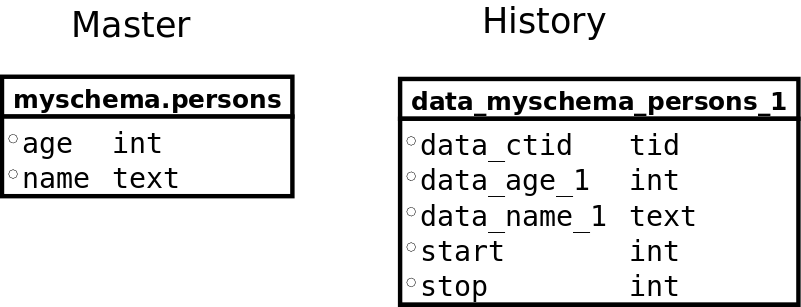
\includegraphics[width=0.6\textwidth]{history-data-table}
  \caption{An example of the schema of a data table in the history database}
  \label{fig:history-data-table-2}
\end{figure}

Marty creates all data tables in the master schema of the history database.
To avoid naming conflicts new names are creates for them: \textit{data\_[schema]\_[table]\_[version]}.
They all have the prefix \textit{data\_} followed by the name of the schema they are part of in the slave database.
Next comes the name of the original table and the name ends with the ID of the history version where this table was created.
This makes it possible for Marty to keep all the data tables in one schema in the history database, even if more than one table from different schemas share the same name in the slave database.
It also handles name reuse when a table is dropped and another table is created with the same name.
These two tables are not part of the same history version and thus the names of the data tables are different.

\begin{figure}[h]
  \centering
    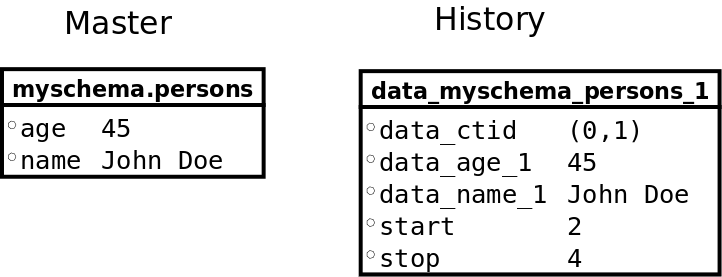
\includegraphics[width=0.6\textwidth]{history-data-table-contents}
  \caption{An example of the data in a data table in the history database}
  \label{fig:history-data-table-contents}
\end{figure}

The columns of the data tables use similar names.
They have the \textit{data\_} prefix and are suffixed with the history version where they were added to the table.
See figure \ref{fig:history-data-table-2} for an example of the schema of a data table in the history database.
Figure \ref{fig:history-data-table-contents} shows an example of the contents of a data table.